\documentclass[12pt]{article}

%%%%%%%%%%%%%%%%%%%%%%%%%%%%%%%%%%%%%%%%%%%%%%%%%%%%%%%%%%%%%%%%%%%%%%%%%%%%%%%%
%                           Package preset for homework
%%%%%%%%%%%%%%%%%%%%%%%%%%%%%%%%%%%%%%%%%%%%%%%%%%%%%%%%%%%%%%%%%%%%%%%%%%%%%%%%
% Miscellaneous
\usepackage[margin=1in]{geometry}
\usepackage[utf8]{inputenc}
\usepackage{indentfirst}
\usepackage{blindtext}
\usepackage{graphicx}
\usepackage{xr-hyper}
\usepackage{hyperref}
\usepackage{enumitem}
\usepackage{color}
\usepackage{float}
% Math
\usepackage{latexsym}
\usepackage{amsfonts}
\usepackage{amssymb}
\usepackage{amsmath}
\usepackage{commath}
\usepackage{amsthm}
\usepackage{bbold}
\usepackage{bm}
% Physics
\usepackage{physics}
\usepackage{siunitx}
% Code typesetting
\usepackage{listings}
% Citation
\usepackage[authoryear]{natbib}
\usepackage{appendix}
\usepackage[capitalize]{cleveref}
% Title & name
\title{Homework}
\author{Tien Vo}
\date{\today}


%%%%%%%%%%%%%%%%%%%%%%%%%%%%%%%%%%%%%%%%%%%%%%%%%%%%%%%%%%%%%%%%%%%%%%%%%%%%%%%%
%                   User-defined commands and environments
%%%%%%%%%%%%%%%%%%%%%%%%%%%%%%%%%%%%%%%%%%%%%%%%%%%%%%%%%%%%%%%%%%%%%%%%%%%%%%%%
%%% Misc
\sisetup{load-configurations=abbreviations}
\newcommand{\due}[1]{\date{Due: #1}}
\newcommand{\hint}{\textit{Hint}}
\let\oldt\t
\renewcommand{\t}[1]{\text{#1}}

%%% Bold sets & abbrv
\newcommand{\N}{\mathbb{N}}
\newcommand{\Z}{\mathbb{Z}}
\newcommand{\R}{\mathbb{R}}
\newcommand{\Q}{\mathbb{Q}}
\let\oldP\P
\renewcommand{\P}{\mathbb{P}}
\newcommand{\LL}{\mathcal{L}}
\newcommand{\FF}{\mathcal{F}}
\newcommand{\HH}{\mathcal{H}}
\newcommand{\NN}{\mathcal{N}}
\newcommand{\ZZ}{\mathcal{Z}}
\newcommand{\RN}[1]{\textup{\uppercase\expandafter{\romannumeral#1}}}
\newcommand{\ua}{\uparrow}
\newcommand{\da}{\downarrow}

%%% Unit vectors
\newcommand{\xhat}{\vb{\hat{x}}}
\newcommand{\yhat}{\vb{\hat{y}}}
\newcommand{\zhat}{\vb{\hat{z}}}
\newcommand{\nhat}{\vb{\hat{n}}}
\newcommand{\rhat}{\vb{\hat{r}}}
\newcommand{\phihat}{\bm{\hat{\phi}}}
\newcommand{\thetahat}{\bm{\hat{\theta}}}

%%% Other math stuff
\providecommand{\units}[1]{\,\ensuremath{\mathrm{#1}}\xspace}
% Set new style for problem
\newtheoremstyle{problemstyle}  % <name>
        {10pt}                   % <space above>
        {10pt}                   % <space below>
        {\normalfont}           % <body font>
        {}                      % <indent amount}
        {\bfseries\itshape}     % <theorem head font>
        {\normalfont\bfseries:} % <punctuation after theorem head>
        {.5em}                  % <space after theorem head>
        {}                      % <theorem head spec (can be left empty, 
                                % meaning `normal')>

% Set problem environment
\theoremstyle{problemstyle}
\newtheorem{problemenv}{Problem}[section]
\newenvironment{problem}[1]{%
  \renewcommand\theproblemenv{#1}%
  \problemenv
}{\endproblemenv}
% Set lemma environment
\newenvironment{lemma}[2][Lemma]{\begin{trivlist}
\item[\hskip \labelsep {\bfseries #1}\hskip \labelsep {\bfseries #2.}]}{\end{trivlist}}
% Set solution environment
\newenvironment{solution}{
    \begin{proof}[Solution]$ $\par\nobreak\ignorespaces
}{\end{proof}}
\numberwithin{equation}{problemenv}

%%% Page format
\setlength{\parindent}{0.5cm}
\setlength{\oddsidemargin}{0in}
\setlength{\textwidth}{6.5in}
\setlength{\textheight}{8.8in}
\setlength{\topmargin}{0in}
\setlength{\headheight}{18pt}

%%% Code environments
\definecolor{dkgreen}{rgb}{0,0.6,0}
\definecolor{gray}{rgb}{0.5,0.5,0.5}
\definecolor{mauve}{rgb}{0.58,0,0.82}
\lstset{frame=tb,
  language=Python,
  aboveskip=3mm,
  belowskip=3mm,
  showstringspaces=false,
  columns=flexible,
  basicstyle={\small\ttfamily},
  numbers=none,
  numberstyle=\tiny\color{gray},
  keywordstyle=\color{blue},
  commentstyle=\color{dkgreen},
  stringstyle=\color{mauve},
  breaklines=true,
  breakatwhitespace=true,
  tabsize=4
}
\lstset{
  language=Mathematica,
  numbers=left,
  numberstyle=\tiny\color{gray},
  numbersep=5pt,
  breaklines=true,
  captionpos={t},
  frame={lines},
  rulecolor=\color{black},
  framerule=0.5pt,
  columns=flexible,
  tabsize=2
}


\title{Homework 6: Phys 5210 (Fall 2021)}

\begin{document}
\maketitle
%%%%%%%%%%%%%%%%%%%%%%%%%%%%%%%%%%%%%%%%%%%%%%%%%%%%%%%%%%%%%%%%%%%%%%%%%%%%%%%%
\begin{problem}{1}
Consider a rigid body (of uniform density and mass $m$) in the shape of a cone
of the base of radius $R$ and height $h$. Find its principal moments of inertia
relative to its center of mass.
\begin{solution}
\begin{center}
    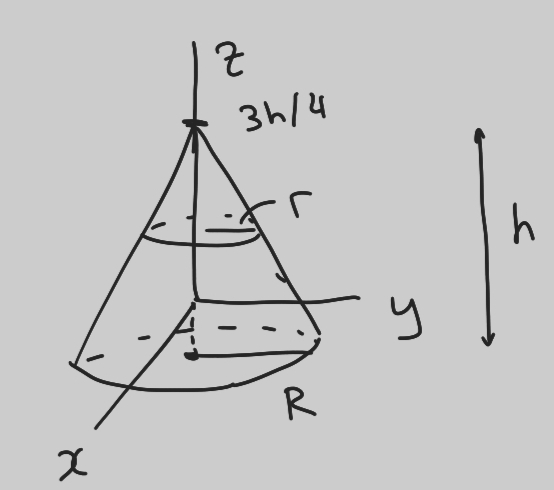
\includegraphics[width=0.5\textwidth]{hw6_p1.jpg} 
\end{center}
Place the cone in a coordinate system as shown above. By geometry, for a given
$r\in[0,R]$, $-h /4\leq z\leq h(3 /4-r /R)$. Then the center of mass is at
\begin{equation}
    z_{cm}=\frac{\rho}{m}
        \int_0^R\int_0^{2\pi}\int_{-h/4}^{h(3/4-r/R)}rdzd\varphi dr
    =0
\end{equation}
By definition, the moment of inertia tensor is
\begin{align}
    \vb{I}&=\rho\int_Vrdrd\varphi dz\mqty(
        y^2+z^2 & -xy & -xz\\
        -xz & x^2 + z^2 & -yz\\
        -xz & -yz & x^2+y^2
    )\notag\\
    &=\rho\int_Vrdrd\varphi dz\mqty(
        r^2\sin^2\varphi+z^2 & -r^2\sin\varphi\cos\varphi & -rz\cos\varphi\\
        -r^2\sin\varphi\cos\varphi & r^2\cos^2\varphi+z^2 & -rz\sin\varphi\\
        -rz\cos\varphi & -rz\sin\varphi & r^2
    )
\end{align}
Note that the off-diagonal terms here all vanish under the azimuthal
integration because $\sin\varphi\cos\varphi,\sin\varphi,\cos\varphi$ are all odd
functions of $\varphi$ in an even domain $[0,2\pi]$. Now we can calculate the
diagonal terms
\begin{align}
    I_{xx}
    &=\rho\int_0^R\int_{-h/4}^{h(3/4-r/R)}\int_0^{2\pi}
        (r^3\sin^2\varphi+rz^2)d\varphi
    dzdr\notag\\
    &=\pi\rho\int_0^R\int_{-h/4}^{h(3/4-r/R)}(r^3+2rz^2)dzdr\notag\\
    &=\rho\frac{\pi}{80}hR^2(h^2+4R^2)\notag\\
    &=3m\qty(\frac{R^2}{20}+\frac{h^2}{80})
\end{align}
where $\rho=m /(\pi hR^2 /3)$. Now, also note that
\begin{align}
    I_{yy}=\rho\int_0^R\int_{-h/4}^{h(3/4-r/R)}\int_0^{2\pi}
        (r^3\cos^2\varphi+rz^2)d\varphi dzdr
          =\rho\int_0^R\int_{-h/4}^{h(3/4-r/R)}(r^3+2rz^2)dzdr
          =I_{xx}
\end{align}
This makes sense because a cone is a symmetric top. Finally,
\begin{align}
    I_{zz}
    =2\pi\rho\int_0^R\int_{-h/4}^{h(3/4-r/R)}r^3dzdr
    =\rho\frac{\pi}{10}hR^4
    =\frac3{10}mR^2
\end{align}
\end{solution}
\end{problem}
%%%%%%%%%%%%%%%%%%%%%%%%%%%%%%%%%%%%%%%%%%%%%%%%%%%%%%%%%%%%%%%%%%%%%%%%%%%%%%%%    
%%%%%%%%%%%%%%%%%%%%%%%%%%%%%%%%%%%%%%%%%%%%%%%%%%%%%%%%%%%%%%%%%%%%%%%%%%%%%%%%
\begin{problem}{2}
(a) A symmetric top is attached by a point to a support which cannot move but
can allow the top to move freely as long as the point remains fixed, as shown in
the Figure. The top is spinning about its symmetry axis, and simmultaneously its
symmetry axis undergoes some motion about the $z$ axis. Its moments of inertia
are $I_3$, as well as $I_1=I_2$, its mass is $m$, and the distance between the
fixed point and the center of inertia is $a=h /\cos\theta$, where $h$ and
$\theta$ are shown in the Figure. Solve the equations of motion of the symmetric
top ``in quadrature'', that is, in terms of integrals as opposed to differential
equations. You don't have to evaluate the integrals you will get.

\begin{center}
    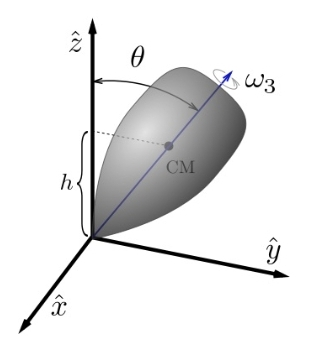
\includegraphics[width=0.3\textwidth]{hw6_p2.jpg} 
\end{center}

The solution of this part of the problem can follow Section 5.7 of Goldstein.
The following strategy may be useful: write down the Lagrange function in terms
of the Euler angles, identify ``cyclic'' variables, that is, the ones where the
Lagrange function depends only on the time derivatives, or velocities, of these
variables, and not on the variables themselves. Use that to identify conserved
quantities, as well as use conservation of energy to arrive at a single first
order differential equation for a single Euler angle which can be solved in
terms of an integral.

(b) Now apply this formalism to the motion of a symmetric top which is freely
suspended in space. We already know that this motion consists of the top
rotating about its symmetry axis, and the symmetry axis rotating about the
direction of the conserved angular momentum. The goal is to reproduce this
behavior from the equations derived in the previous section. Modify these
equations to describe motion of a symmetric top relative to its center of mass
(as opposed to the fixed point of the previous section). Point the conserved
angular momentum along the vertical axis. The motion of a free top should then
correspond to $\theta=\text{const}$. Analyze the equations of motion to find the
condtions making constant $\theta$ possible, and find the angular velocity of
the rotation of the axis of the top about the direction of angular momentum
$\Omega_{pr}$, as well as the angular velocity of its spinning about its
symmetry axis $\Omega_3$ ($\omega_3$ in the figure above) in terms of $\theta$
and the magnitude of its angular momentum $l$.
\begin{solution}
(a) The potential of the top is $U=mga\cos\theta$. Thus, we can write the
Lagrange function in terms of Euler angles as
\begin{equation}
    \LL
    =\frac12I_1\Omega_1^2+\frac12I_2\Omega_2^2+\frac12I_3\Omega_3^2-U
    =\frac{I_1}{2}\qty(\dot\theta^2+\dot\varphi^2\sin^2\theta) 
    +\frac{I_3}{2}\qty(\dot\psi+\dot\varphi\cos\theta)^2-mga\cos\theta
\end{equation}
where
\begin{subequations}\label{p2a:euler_angles}
    \begin{align}
        \Omega_1&=\dot\theta\cos\psi+\dot\varphi\sin\theta\sin\psi\\
        \Omega_2&=-\dot\theta\sin\psi+\dot\varphi\sin\theta\cos\psi\\
        \Omega_3&=\dot\psi+\dot\varphi\cos\theta
    \end{align}
\end{subequations}
From Euler-Lagrange equations, we find the integrals ($P_\psi,P_\varphi$) of the
motion
\begin{subequations}\label{p2a:P}
    \begin{align}
        \frac{\partial\LL}{\partial\dot\psi}
        &=I_3(\dot\psi+\dot\varphi\cos\theta)=P_\psi=I_3\Omega_3\\
    \frac{\partial\LL}{\partial\dot\varphi}
        &=(I_1\sin^2\theta+I_3\cos^2\theta)\dot\varphi+I_3\cos\theta\dot\psi
        =P_\varphi
    \end{align}
\end{subequations}
These are conserved because $\LL$ is independent of $\psi$ and $\varphi$. Then 
we can solve the system of equations \eqref{p2a:P} for the conserved
angular velocities $\dot\varphi$ and $\dot\psi$
\begin{subequations}\label{p2a:dot}
    \begin{align}
        \dot\psi&=\qty(1+\frac{I_3}{I_1}\cot^2\theta)\Omega_3
        -\frac{\cot\theta\csc\theta}{I_1}P_\varphi\\
        \dot\varphi&=\frac{P_\varphi-I_3\Omega_3\cos\theta}{I_1\sin^2\theta}
        \label{p2a:varphidot}
    \end{align} 
\end{subequations}
Now, the total energy of the top is,
\begin{align}
    E
    &=\frac12I_1(\dot\theta^2+\dot\varphi^2\sin^2\theta)
    +\frac12I_3\qty(\dot\psi+\dot\varphi\cos\theta)^2+mga\cos\theta \notag\\
    &=\frac12I_1(\dot\theta^2+\dot\varphi^2\sin^2\theta)
    +\frac12I_3\Omega_3^2+mga\cos\theta
\end{align}
This is a sole function of $\theta$, as indicated by \eqref{p2a:dot}. Thus, we
can invert and write the following ordinary differential equation of $\theta$
\begin{equation}\label{p2a:ODE1}
    \dot\theta=\qty[\frac{2E-I_3\Omega_3^2}{I_1}-\frac{2mga}{I_1}\cos\theta
    -\frac{\qty(P_\varphi-I_3\Omega_3\cos\theta)^2}{I_1^2\sin^2\theta}]^{1/2} 
\end{equation}
Letting $\alpha=(2E-I_3\Omega_3^2) /I_1,\beta=2mga /I_1,b=P_\varphi /I_1,$ and
$c=I_3\Omega_3 /I_1$. \eqref{p2a:ODE1} can then be rewritten as
\begin{equation}\label{p2a:thetadot}
    \dot\theta=\sqrt{\alpha-\beta\cos\theta-\frac{(b-c\cos\theta)^2}{\sin^2\theta}} 
\end{equation}
Let $u=\cos\theta$, then this differential equation becomes
\begin{equation}
    \dot{u}=\sqrt{(1-u^2)(\alpha-\beta u)-(b-cu)^2} 
\end{equation}
which can be solved in quadrature as
\begin{equation}
    t=\int_{u(0)}^{u(t)}\frac{du}{\sqrt{(1-u^2)(\alpha-\beta u)-(b-cu)^2}} 
\end{equation}

(b) Note that $L_1=I_1\Omega_1=l\sin\theta\sin\psi$ and
$L_2=I_2\Omega_2=l\sin\theta\cos\psi$. So we can calculate the precession
(rotation around $\zhat$) from \eqref{p2a:euler_angles} as
\begin{equation}
    \Omega_{pr}=\dot\varphi=\frac{I_1\sin\psi+\Omega_2\cos\psi}{\sin\theta} 
    =\frac{I_1\Omega_1^2+I_2\Omega_2^2}{l\sin^2\theta}
    =l\frac{I_1\Omega_1^2+I_2\Omega_2^2}{I_1^2\Omega_1^2+I_2\Omega_2^2}
\end{equation}
For a symmetric top, $I_1=I_2$ and we can write
\begin{equation}\label{p2b:precession}
    \Omega_{pr}=\frac{l}{I_1} 
\end{equation}

Now, for a gyroscope, $\beta=0$ and \eqref{p2a:thetadot} is
\begin{equation}
    \dot\theta=\sqrt{\alpha-\frac{(b-c\cos\theta)^2}{\sin^2\theta}} 
\end{equation}
The condition for $\dot\theta=0$ is then
\begin{equation}
    \sqrt{\alpha}=\frac{b-c\cos\theta}{\sin\theta} 
\end{equation}
However, from \eqref{p2a:varphidot},
\begin{equation}\label{p2b:varphidot}
    \dot\varphi=\frac{b-c\cos\theta}{\sin^2\theta}=\frac{\sqrt\alpha}{\sin\theta}
\end{equation}
Combining \eqref{p2b:precession} and \eqref{p2b:varphidot}
($\Omega_{pr}=\dot\varphi$), we have
\begin{equation}\label{p2b:alpha}
    \alpha=\frac{l^2\sin^2\theta}{I_1^2} 
\end{equation}
By definition, the angular momentum is
\begin{equation}
    \vb{L}=I_1\Omega_1\hat{n_1}+ I_2\Omega_2\hat{n_2}+ I_3\Omega_3\hat{n_3}
\end{equation}
Thus,
\begin{equation}
    l^2=I_1^2(\Omega_1^2+\Omega_2^2)+I_3^2\Omega_3^2 
    =I_1^2\dot\varphi^2\sin^2\theta+I_3^2\Omega_3^2
    =I_1^2\alpha+I_3^2\Omega_3^2
\end{equation}
where we have used the Euler angle defintions \eqref{p2a:euler_angles} in the
second equality and \eqref{p2b:varphidot} in the third equality. Plugging
\eqref{p2b:alpha} into this result, we can invert and solve for $\Omega_3$
\begin{equation}
    l^2=l^2\sin^2\theta+I_3^2\Omega_3^2\Rightarrow\Omega_3=\frac{l\cos\theta}{I_3} 
\end{equation}

\end{solution}
\end{problem}
%%%%%%%%%%%%%%%%%%%%%%%%%%%%%%%%%%%%%%%%%%%%%%%%%%%%%%%%%%%%%%%%%%%%%%%%%%%%%%%%
\end{document}
